\section{Results \& Evaluations}
In this chapter, we perform evaluation on our model and the other algorithms, the repository of our model is provided in github \footnote{\url{https://github.com/cwleung/LKJTM}}.
\subsection{Experiment Testing}
The experiment will be conducted with a number of existing proposed topic models as mentioned related work section above. We conduct the experiment with those baseline algorithms and evaluate them in terms of accuracy and running time. Some of the source code of competitive were provided by their authors in Github\footnote{For instance, Correlated Topic Model(CTM), \href{https://github.com/blei-lab/ctm-c}{https://github.com/blei-lab/ctm-c}}. The outcome result will be extensively studied and conclude the insight behind the algorithms and methodologies. Detail to be stated in section \ref{AD}. Our probabilistic part of model implemented using Pyro\cite{bingham_pyro_2019}, while the model optimization and transformer implementations are based on PyTorch\cite{paszke_automatic_2017}.
\subsection{Dataset}To evaluate the performance of the model, we select the two most poplar data set in the context of topic model evaluation. 20Newsgroups and Reuter RCV1-v2 datasets. 20NewsGroup consist of 18,846 news group documents \footnote{\url{http://qwone.com/~jason/20Newsgroups/}} and the RCV1-v2 includes 10,000 documents in total. Both of the dataset will be preprocessed to remove stopwords and stemming before the evaluation. If desirable, it will also to be applied to NIST TREC dataset and NII NTCIR dateset for further application studies.
\subsection{Data Preprocessing}
We perform data preprocessing, tokenization, stopword removal, lemmatization, and set the 
\subsection{Models}
We compare the model performance with a numbers of rivals. We take Latent Dirichlet Allocation (LDA)\cite{blei_latent_2003} as the baseline model. Other models include Transformer\cite{vaswani_attention_nodate}\footnote{Not a topic model, but we think it is worth to make comparison still.},  ProdLDA\cite{srivastava_autoencoding_2017} and Embedded Topic Model(ETM)\cite{dieng_topic_2019}.
\subsection{Algorithmic Settings}
% optimization algorithm
To perform posterior inference, we employed Stochastic Variational Inference (SVI) \cite{hoffman_stochastic_2013} for the optimization problem. We set the minibatch size to 1024 documents.
% Other model
For LDA, we applied the model provided from sklearn package (version 0.24.0) \footnote{Sklearn website \url{https://scikit-learn.org/stable/index.html}}. For ETM, we run the experiment with the parameter suggested \cite{dieng_topic_2019}. For ProdLDA, we perform optimization with inference network architecture as described in the paper \cite{srivastava_autoencoding_2017}. 
% learning rate
To perform optimization, we use Adam for the gradient ascent algorithm, and we set the learning rate to 1e-3.
% l2-regularization factor
we use $ l2 $-regularization to the 
% inference network [size, activation function, dropout, batch-norm]
We use 
% Transformer settings

% 
\subsection{Quantitative Result}
In this section, we evaluate the model with the following metric adopted from \cite{dieng_dynamic_2019}: Perplexity, Topic Coherence (TC), Topic Diversity (TD). %and Topic Quality (TQ).\begin{center}
\begin{table}[h]
\centering
\begin{tabular}{llll}
\hline
Model      & TC     & Perplexity  \\ \hline
Transformer & -0.311 & - \\
LDA & 0.183 & 2425.9 \\
ProdLDA		&  0.107 & 5652.0\\
ETM	     	&  0.177 & \textbf{1919.3}\\
\textbf{Our model}  & \textbf{0.206} & 3444.1 \\ \hline
\end{tabular}
\label{tbl:t1}
\caption{Result of our implementation(topic k=20)}
\end{table}
\begin{table}[h]
\centering
\begin{tabular}{llll}
\hline
Model      & TC     & Perplexity  \\ \hline
Transformer & -0.251 & - \\
LDA & 0.155 & \textbf{2536.1} \\
ProdLDA		&  0.074 & 5654.1\\
ETM	     	&  0.145 & 2603.9\\
\textbf{Our model}  & \textbf{0.199} & 3705.0 \\ \hline
\end{tabular}
\label{tbl:t2}
\caption{Result of our implementation(topic k=50)}
\end{table}
\paragraph{Discussion}On the result from table \ref{fig:eval_20ng_20t}, \ref{fig:eval_20ng_50t}, display that our model has outperform the other model by TC score. On perplexity score, ETM obtain the best score when $ k=20 $ and LDA when $ k=50 $. Since Transformer is not a topic model actually, it got a negative score on TC, which refers it cannot retrieve any useful topic from documents.
\subsection{Training}
From figure \ref{fig:loss_20ng_20t}, \ref{fig:loss_20ng_50t}, display the training process of the training loss and log probability by 200 epochs. From \ref{fig:eval_20ng_20t}, \ref{fig:eval_20ng_50t}, we observe that the TD score and TC score increase monotonically, however, the perplexity increases throughout the epochs. 
\subsection{Qualitative Result}The proposed model will be evaluated with a number of specifically selected topic and examined with their performance separately. The result will be exhaustively compared with other existing models.\\
From table \ref{tbl:t3}, we have selected some topic words each model generated from 20Newsgroups when $ k=20 $. The topics represent space, operating system, religion, encryption and guns respectively. Our model has shown capability on capturing key words from each topic, such as on topic "space": \textit{nasa}, \textit{space}, \textit{jpl}, \textit{moon}, \textit{earth}, \textit{station}, \textit{flight} are the outputs.
\begin{table}[h]
\centering
\begin{tabular}{llll}
\hline
Our Model  \\ \hline
\textbf{nasa }gov \textbf{space jpl moon earth station flight }research digex\\
\textbf{windows window }problem \textbf{dos }running \textbf{file mouse }mit de ms\\
\textbf{god jesus christian }people faith bible time church good things\\
key chip encryption clipper security privacy government keys public escrow\\
gun people control government guns weapons american make clinton state \\ \hline
\hline
ProdLDA  \\ \hline
nasa space gov people station time orbit dc program shuttle \\
scsi drive controller max drives ide senior tape time people \\
god jesus atheists christian bible religion atheism christians word truth \\
key crypto session nt chips chip serial dos keys encrypted \\
gun people god religion writes life morality ohio argument question \\ \hline
\hline
LDA  \\ \hline
space, nasa, gov, access, launch, earth, digex, moon, orbit\\
file, window, program, ftp, files, server, image, graphics, windows\\
god, people, jesus, christian, bible, writes, life, christians, time\\
key, encryption, chip, clipper, keys, security, government, privacy\\
gun, guns, law, police, people, weapons, crime, fbi, control
\\ \hline
\hline
ETM  \\ \hline
space, nasa, gov, mr, president, health, research, year, center\\
windows, file, window, program, files, server, version, dos, image\\
god, people, jesus, christian, israel, bible, jews, christians, israeli\\
key, encryption, chip, clipper, keys, privacy, security, technology, government\\
gun, people, government, law, state, guns, article, weapons, control
\\ \hline
\end{tabular}
\label{tbl:t3}
\caption{Top-9 words for each topic from randomly selected 5 topics}
\end{table}
\begin{figure}[h]
\centering
\subcaptionbox{Log probability}{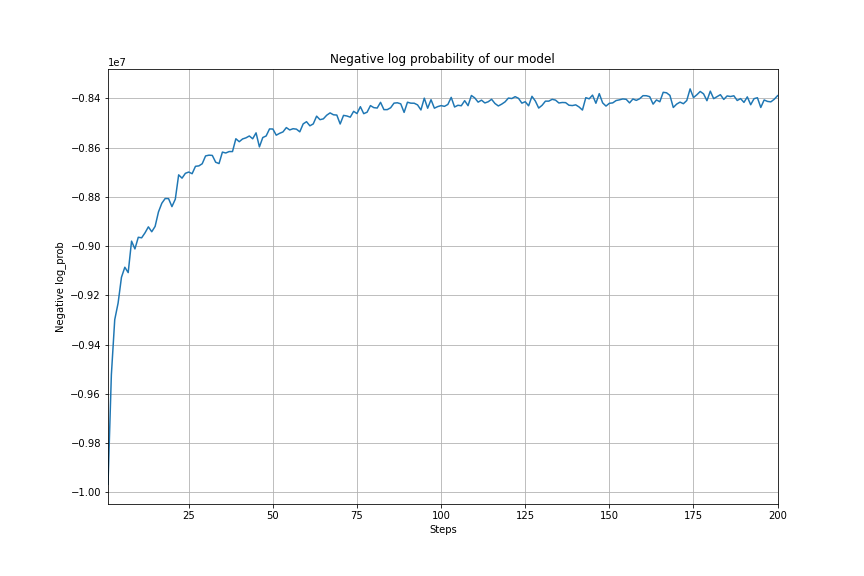
\includegraphics[width=0.50\textwidth]{figure/0908/log_prob_20t}}%
\hfill
\subcaptionbox{Negative ELBO}{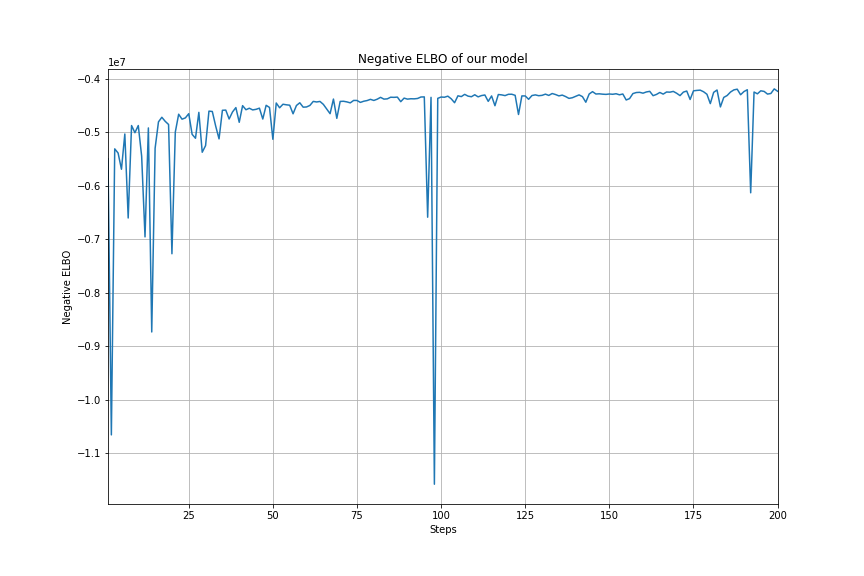
\includegraphics[width=0.50\textwidth]{figure/0908/elbo_20t}}%
\hfill
\caption{20Newsgroups (k=20)}
\label{fig:loss_20ng_20t}
\end{figure}
\begin{figure}
\centering
\subcaptionbox{Log probability}{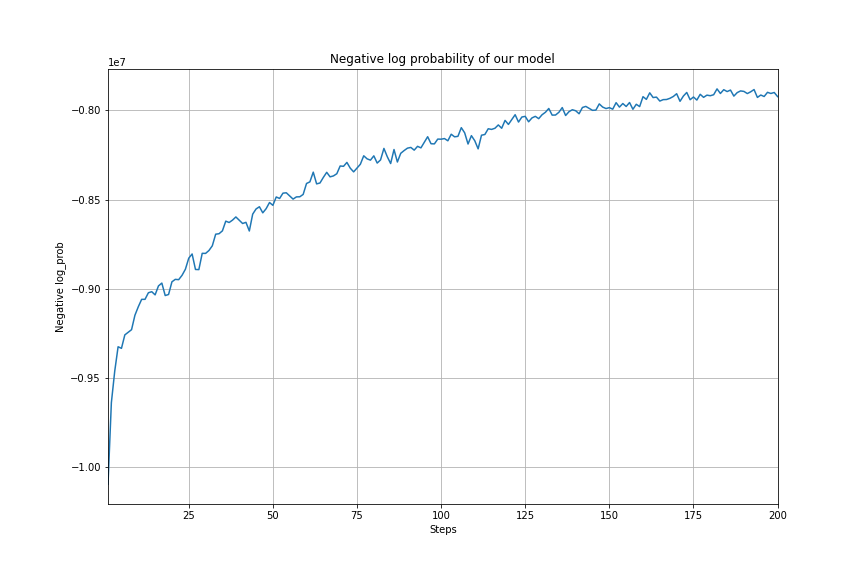
\includegraphics[width=0.50\textwidth]{figure/0908/log_prob_50t}}%
\hfill
\subcaptionbox{Negative ELBO}{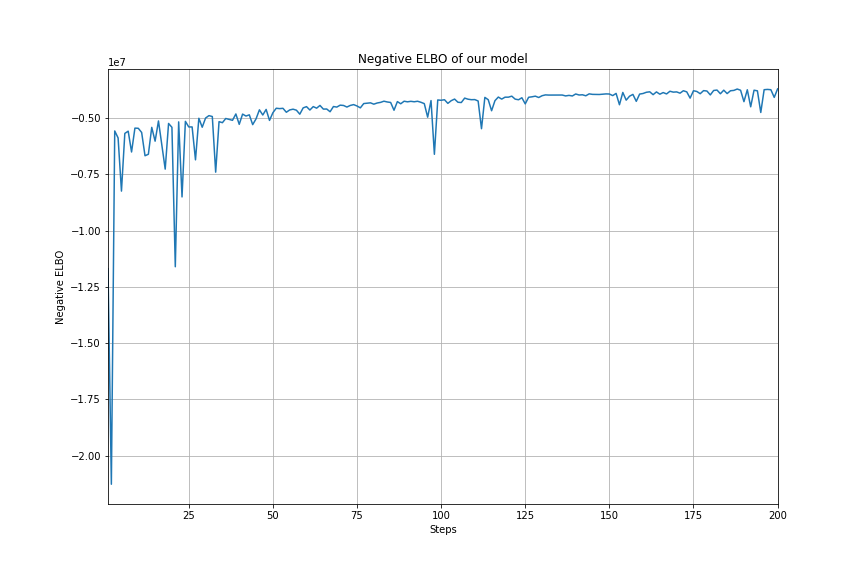
\includegraphics[width=0.50\textwidth]{figure/0908/elbo_50t}}%
\hfill
\caption{20Newsgroups (k=50)}
\label{fig:loss_20ng_50t}
\end{figure}
\begin{figure}
\centering
\subcaptionbox{Topic Diversity}{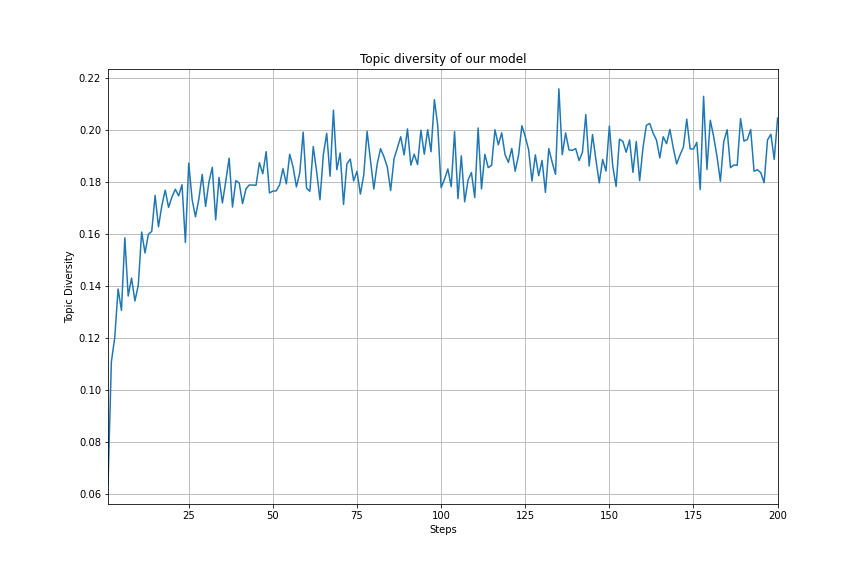
\includegraphics[width=0.50\textwidth]{figure/0908/td_20t}}%
\hfill
\subcaptionbox{Topic Coherence}{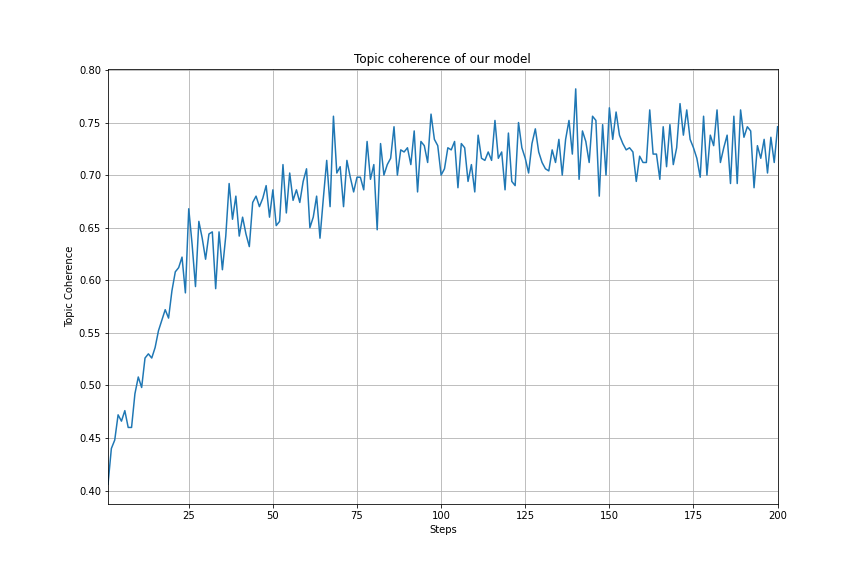
\includegraphics[width=0.50\textwidth]{figure/0908/tc_20t}}%
\hfill
\subcaptionbox{Perplexity}{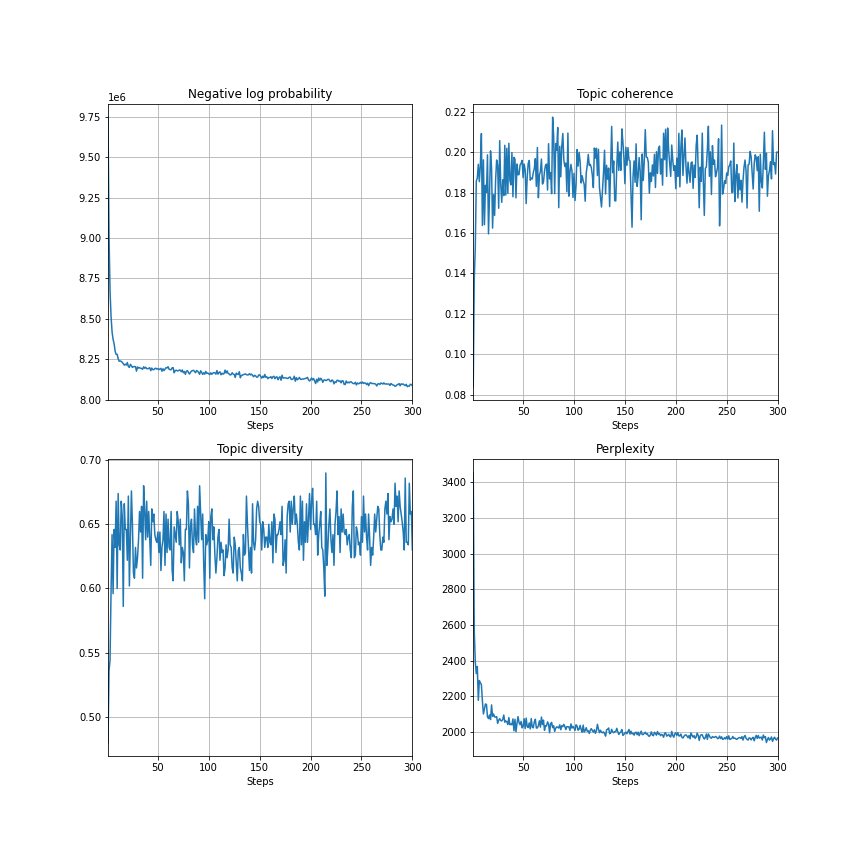
\includegraphics[width=0.50\textwidth]{figure/0908/ppl_20t}}%
\hfill
\caption{20Newsgroups (k=20)}
\label{fig:eval_20ng_20t}
\end{figure}
\begin{figure}
\centering
\subcaptionbox{Topic Diversity}{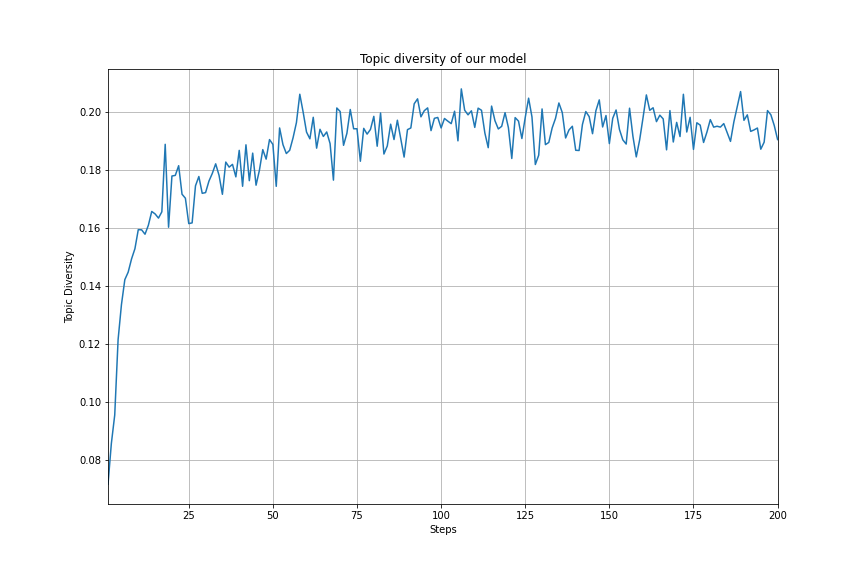
\includegraphics[width=0.50\textwidth]{figure/0908/td_50t}}%
\hfill
\subcaptionbox{Topic Coherence}{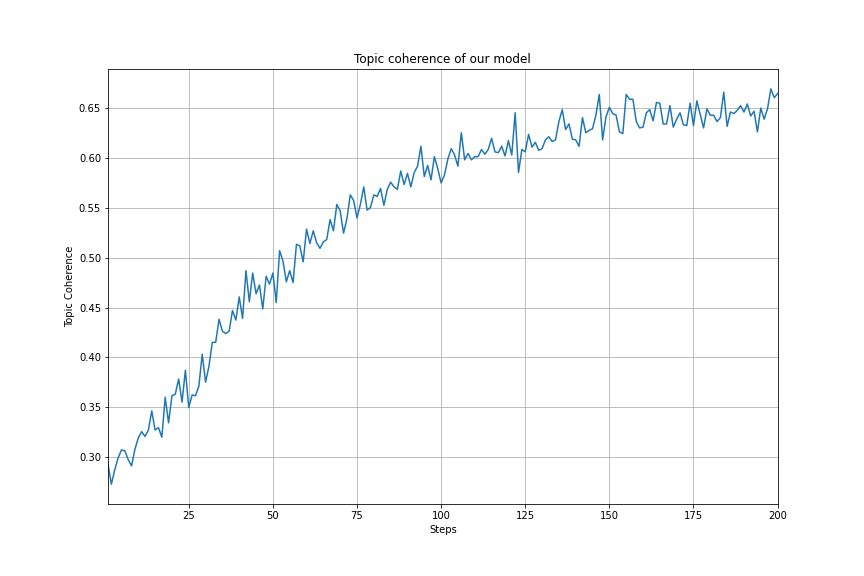
\includegraphics[width=0.50\textwidth]{figure/0908/tc_50t}}%
\hfill
\subcaptionbox{Perplexity}{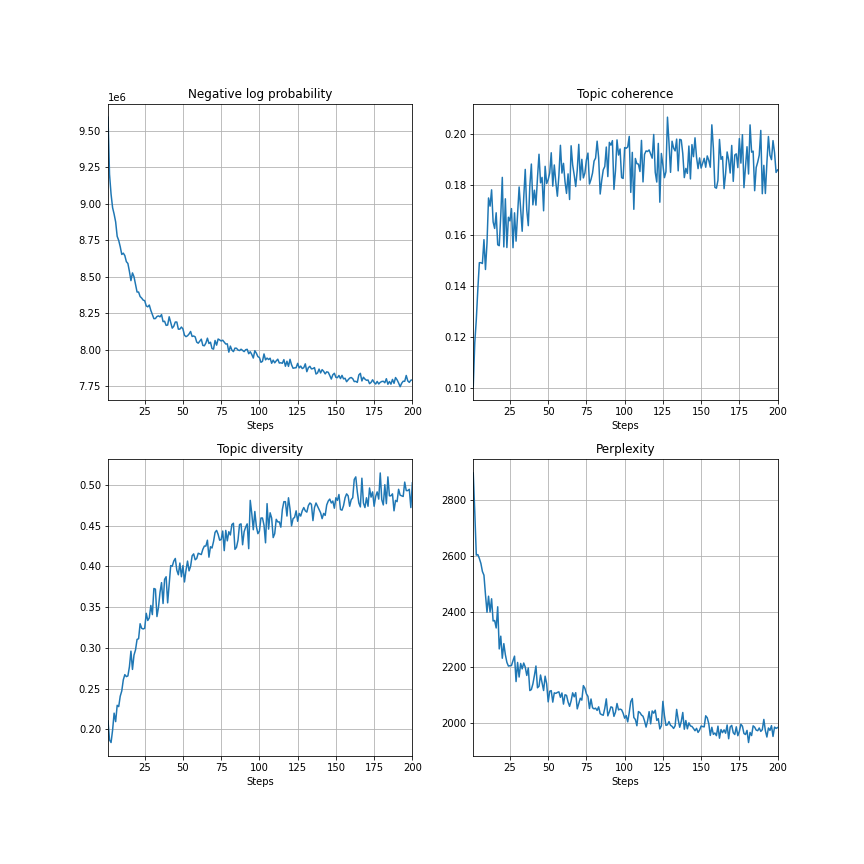
\includegraphics[width=0.50\textwidth]{figure/0908/ppl_50t}}%
\hfill
\caption{20Newsgroups (k=50)}
\label{fig:eval_20ng_50t}
\end{figure}
\subsection{Visualization}
To clearly demonstrate the representation for , we applied t-SNE to map the topic-word representation into 2-dimension continuous space. In figure \ref{fig:tsne20t25w2} and \ref{fig:tsne50t25w0}, demonstrate the t-SNE visualization of the topic-word distribution for 20Newsgroups. 
\begin{figure}
\centering
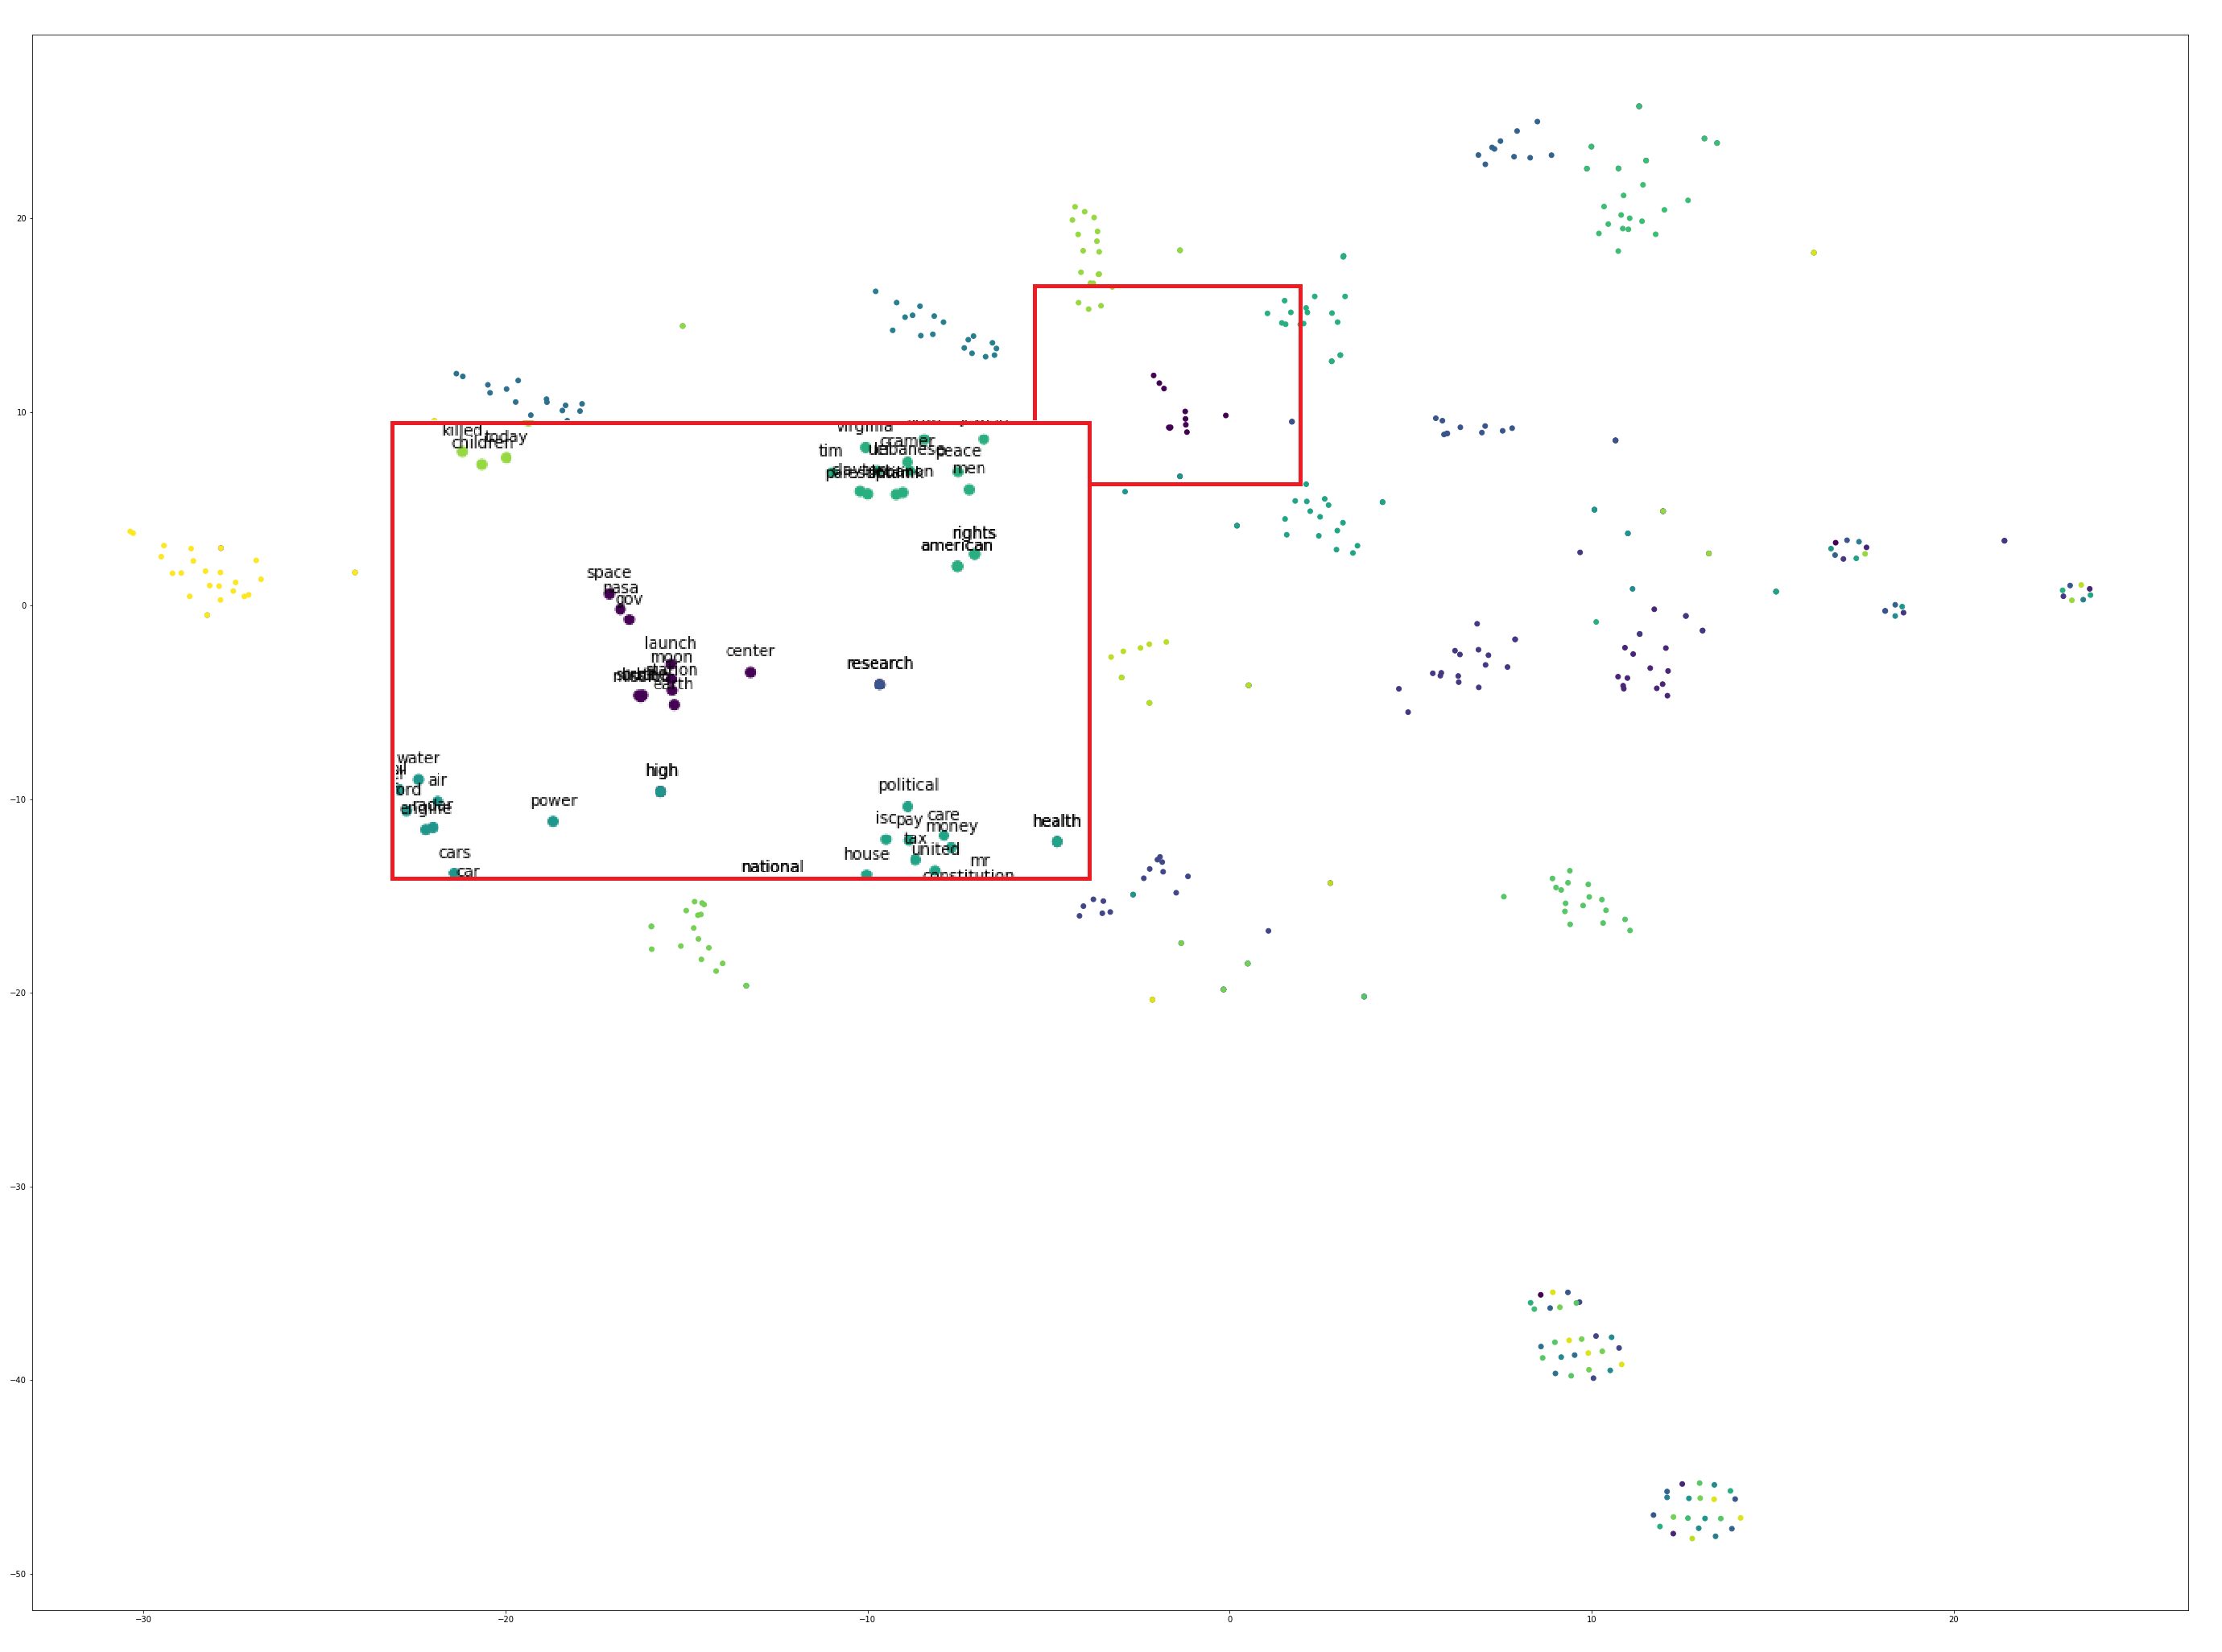
\includegraphics[width=1\linewidth]{figure/0908/tsne_20t_25w_2}
\caption{Visualization \#Topics:20}
\label{fig:tsne20t25w2}
\end{figure}
\begin{figure}
\centering
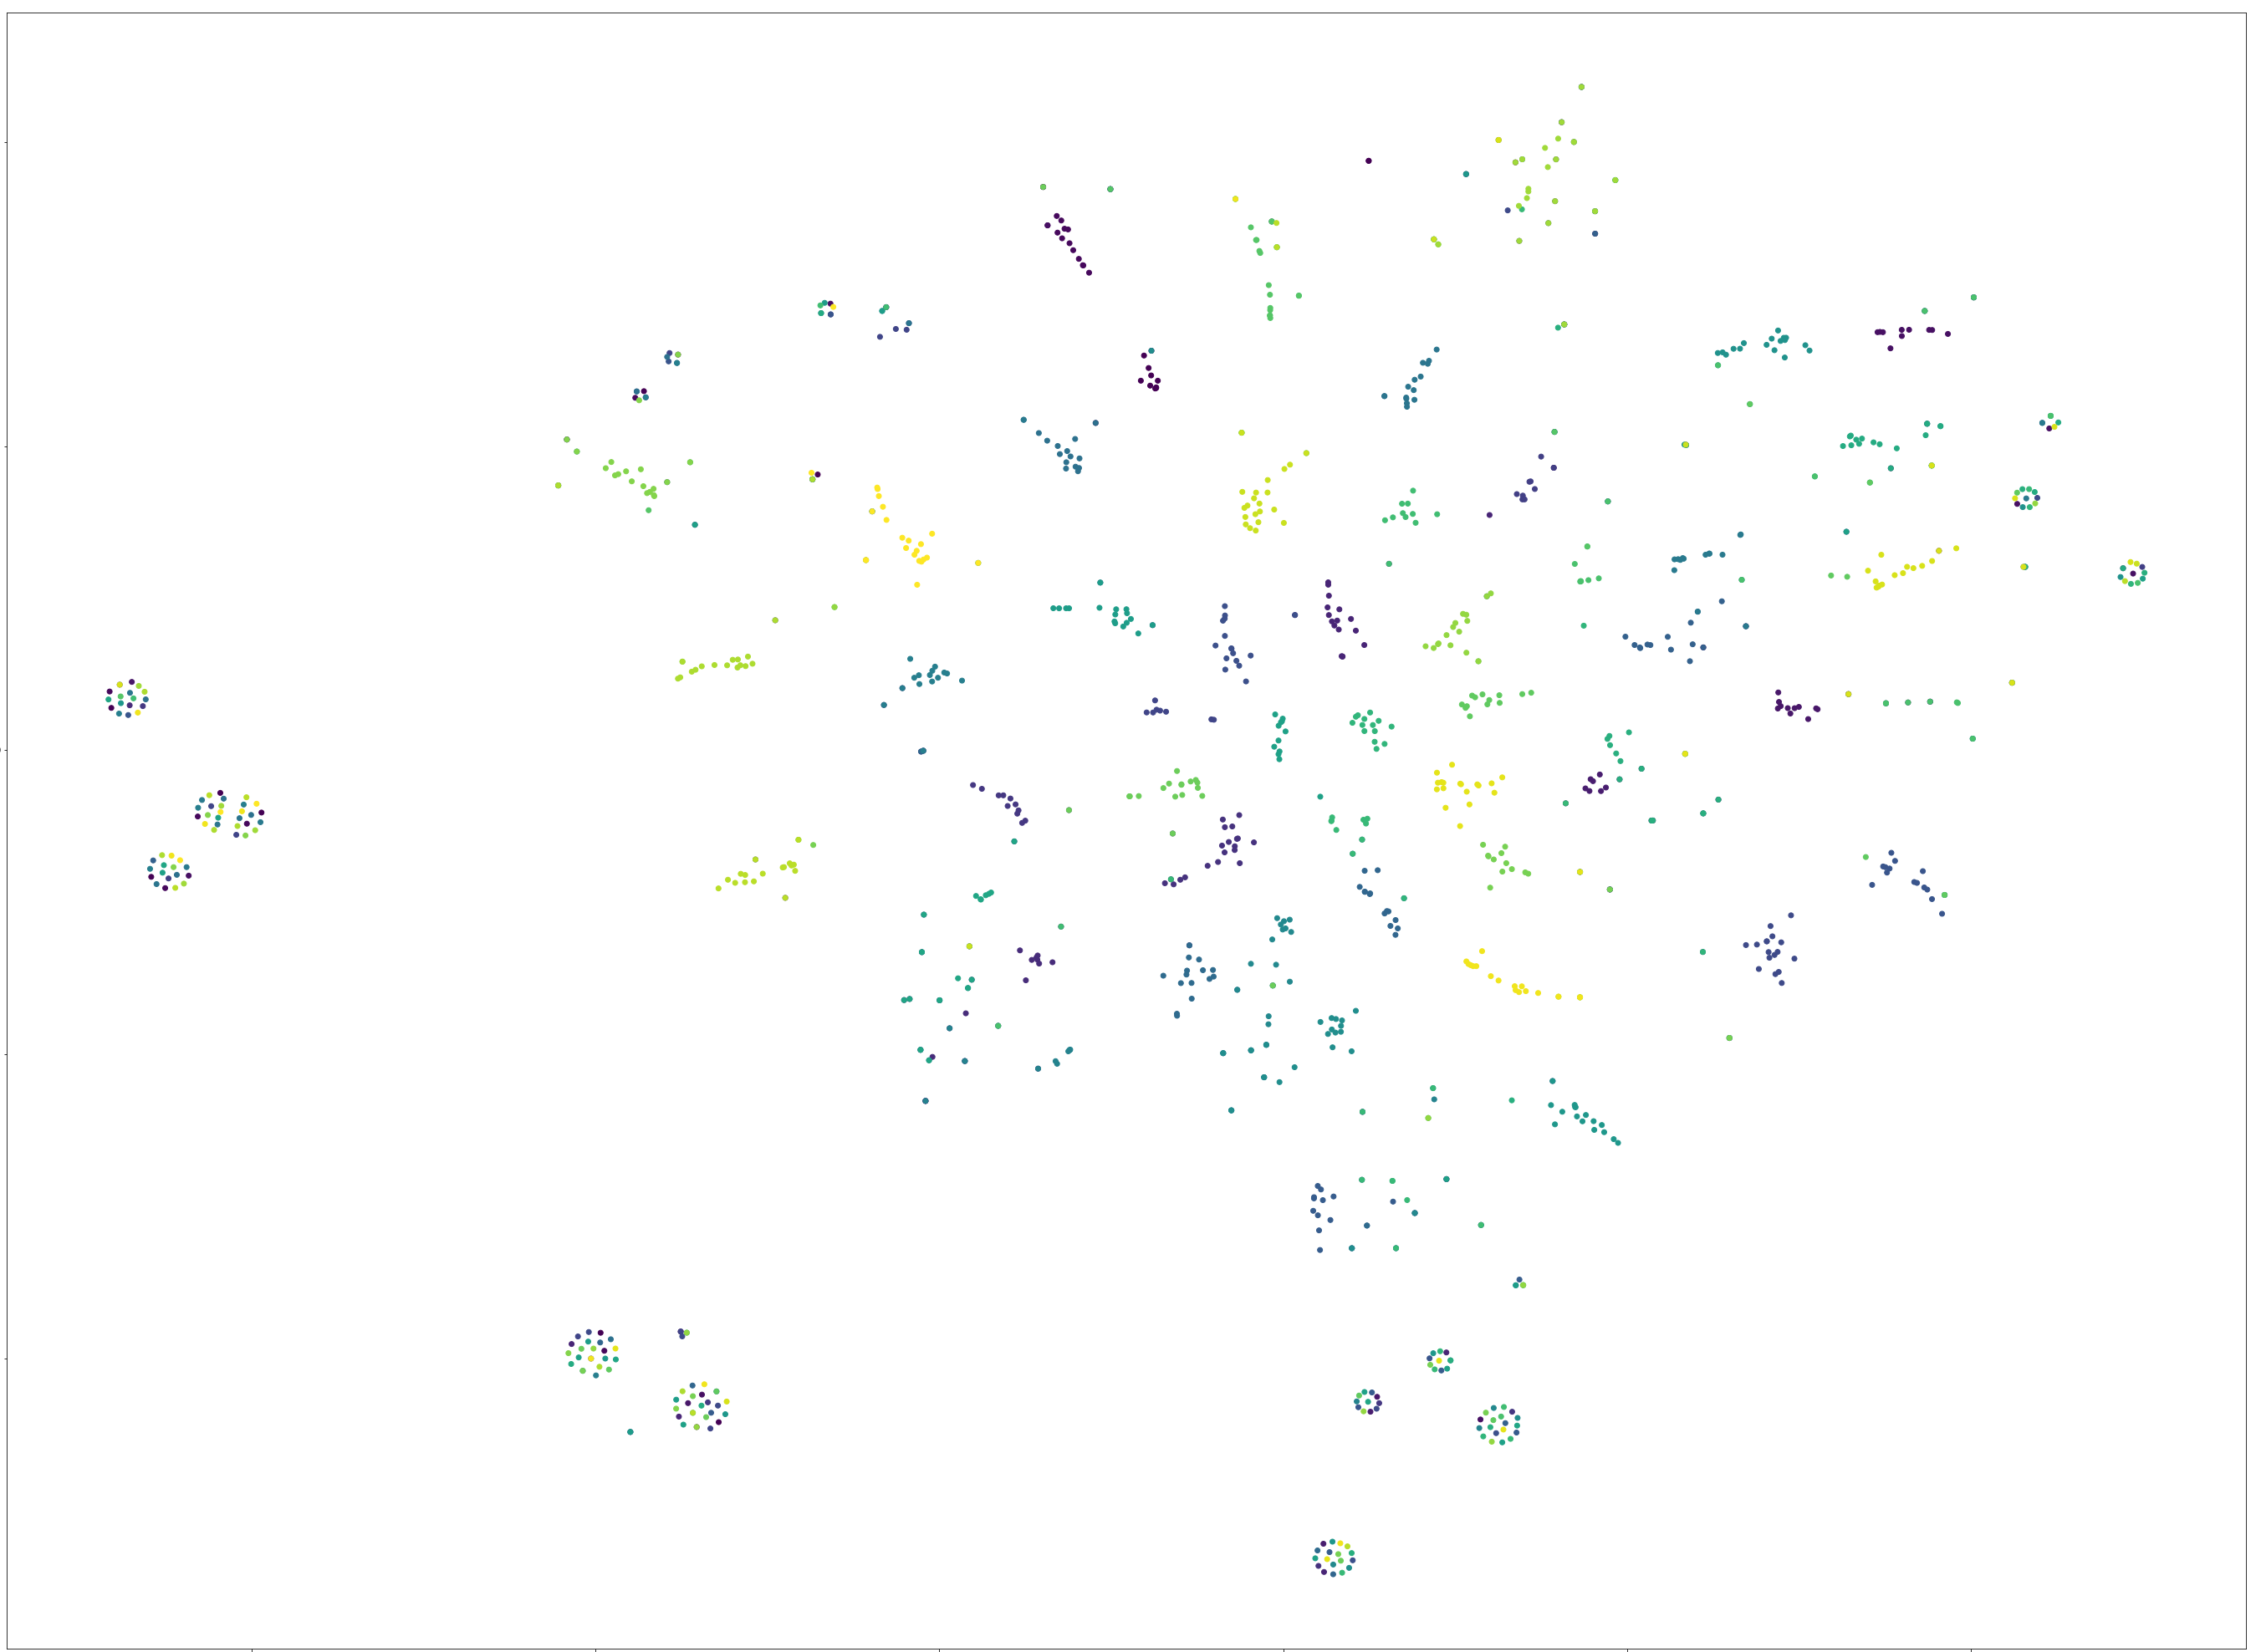
\includegraphics[width=1\linewidth]{figure/0908/tsne_50t_25w_0}
\caption{Visualization \#Topics:50}
\label{fig:tsne50t25w0}
\end{figure}
